\documentclass[a4paper]{article}
\usepackage[margin=3cm]{geometry}
\usepackage{xcolor}
\usepackage{graphicx}
\usepackage{lipsum}
\usepackage{amsmath}
\usepackage{pdfpages}
\usepackage{url}
%\usepackage[backref=page]{hyperref}
\usepackage{hyperref}
\usepackage{subcaption}
\usepackage[font=small,labelfont=bf]{caption}
\usepackage{siunitx}
\usepackage{circuitikz}
\hypersetup{
    colorlinks = true,
    colorlinks = false,
	urlcolor = {blue},
%	linkbordercolor = {transparent},
    pdfborder = {0 0 0},
	linkcolor = {blue},
	citecolor = {blue}
}
\usepackage{acronym}
\usepackage[acronym,nomain]{glossaries}
\makeglossaries
\newcommand{\todo}[1]{\textbf{\textcolor{red}{#1}}}
%\newcommand{\td}[1]{\textbf{\textcolor{red}{#1}}}
\newcommand{\td}[1]{\textcolor{red}{#1}}
\newcommand{\me}[1]{\textcolor{gray}{#1}}
\newcommand{\ds}[1]{}
\newcommand{\x}{$\times$}
\newcommand{\picwidth}{0.7\textwidth}

%SI UNITS
\newcommand{\cm}[1]{\SI{#1}{\centi\meter}}
\newcommand{\mm}[1]{\SI{#1}{\milli\meter}}
\newcommand{\mg}[1]{\SI{#1}{\milli\gram}}
\newcommand{\ml}[1]{\SI{#1}{\milli\liter}}
\newcommand{\um}[1]{\SI{#1}{\micro\meter}}
\newcommand{\ul}[1]{\SI{#1}{\micro\liter}}
\newcommand{\minutes}[1]{\SI{#1}{\minute}}
\newcommand{\oc}[1]{\SI{#1}{\degreeCelsius}}
\newcommand{\s}[1]{\SI{#1}{\second}}
\newcommand{\h}[1]{\SI{#1}{\hour}}
\newcommand{\mmps}[1]{\SI{#1}{\milli\meter\per\second}}

%\title{Functional oxide layers for electrical isolation and chemical passivation of steel substrates}
%\title{Optimisation of Zirconium Oxide layers for electrical isolation and chemical passivation of steel substrate}
\title{Particle Swarm Optimisation of Chemical Passivation of Steel Substrate with Zirconium Oxide Layers through Sol-Gel Process}
\author{Johann Dorn}

\begin{document}
\maketitle
\newacronym{zrpro}{\ch{Zr(PrO)4}}{zirconium(IV)propoxide}
\newacronym{acac}{Hacac}{acetylacetone}
\newacronym{acoh}{AcOH}{glacial acetic acid}
\newacronym{buoh}{BuOH}{Butan-1-ol}
\newacronym{ipo}{IPO}{Propan-2-ol}
\newacronym{ito}{ITO}{indium doped tin oxide}
\newacronym{fto}{FTO}{fluorine doped tin oxide}
\newacronym{n2}{\ch{N2}}{nitrogen}
\newacronym{water}{\ch{H2O}}{deionized water}
\newacronym{sds}{SDS}{sodium dodecyl sulfate}
\newacronym{hcl}{HCl}{hydrochloric acid}
\newacronym{h2so4}{\ch{H2SO4}}{sulfuric acid}
\newacronym{naoh}{\ch{NaOH}}{sodium hydroxide}
\newacronym{zro}{\ch{ZrO2}}{zirconium dioxide}
\newacronym{1f}{1F}{one-fold concentrated solution}
\newacronym{2f}{2F}{two-fold concentrated solution}
\newacronym{3f}{3F}{three-fold concentrated solution}
\newacronym{4f}{4F}{four-fold concentrated solution}
\newacronym{5f}{5F}{five-fold concentrated solution}
\newacronym{db}{DB}{doctor blading}
\newacronym{dbc}{DBC}{doctor blade coating}
\newacronym{pv}{PV}{photovoltaic}
%\newacronym{cigs}{CIGS}{copper indium gallium sulfide}
\newacronym{cigs}{CIGS}{\ch{CuIn_{x}Ga_{1-x}Se2}}
%
\newacronym{pvd}{PVD}{physical vapor deposition}
\newacronym{sg}{SG}{sol-gel}
\newacronym{ir}{IR}{infrafred}
\newacronym{nir}{NIR}{near-infrafred}
\newacronym{ft}{FT}{Fourier transform}
\newacronym{sem}{SEM}{scanning electron microscopy}
\newacronym{xrd}{XRD}{X-ray diffraction}
\newacronym{feg}{FEG}{field emission gun}
\newacronym{mfp}{MFP}{mean free path}
%
\newacronym{pso}{PSO}{particle swam optimization}
\newacronym{ml}{ML}{machine learning}
\newacronym{vs}{vs.}{versus}
\newacronym{iv}{I-V}{current-voltage}
%
\newacronym{em}{EM}{electro magnetic}
\newacronym{uv}{UV}{ultraviolet}
\newacronym{vis}{Vis}{visible}
% AI 
\newacronym{ai}{AI}{artificial intelligence}
\newacronym{nn}{ANN}{artificial neural networks}
\newacronym{ga}{GA}{genetic algorithm}
\newacronym{krr}{KRR}{Kernel Ridge Regression}
\newacronym{svm}{SVM}{Support Vector Machine}
% 
\newacronym{doe}{DOE}{design of experiment}
\newacronym{anova}{ANOVA}{Analysis of Variance}
\newacronym{pb}{PB}{Plackett-Burman}
%
\newacronym{emma}{EMMA}{evolutionary model-based multiresponse approach}
\newacronym{mars}{MARS}{multivariate adaptive regression splines}
% RESULTS
\newacronym{mse}{MSE}{mean squared error}
\newacronym{bf}{BF}{basis function}
\newacronym{rf}{RF}{regression function}
\newacronym{gcv}{GCV}{generalized cross validation}
\newacronym{epv}{EPV}{events per predictor variable}




\clearpage
\section*{Abstract}
%1 Satz intro/background
%1 Satz ergebnisse 
%has been used ist meiner Meinung nach eher zu verwenden, wenn man es auch heute noch den Subjekt benutzt, z.B. diese Methode war (ist aber auch heute noch) in diesem und jenem Bereich eingewendet. was used würde ich eher schreiben bei einem konkretem Fall, zB wenn man bei einer bestimmten Studie etwas benutzt hat 
%\lipsum[1]
%\td{
Passivated steel can act as fit substrate for thin-film photovoltaics.
A thin zirconium oxide layer was applied via blade coating onto a steel foil substrate with the goal of getting a homogeneous and insulating layer.
Layers were qualitatively characterized with SEM and XRD and quantitatively charaterized via current-voltage curves.
The process variables (solution concentration, number of layers, coating speed, coating temperature, calcination speed and calcination temperature) were optimized by particle swarm optimization (PSO) algorithm in combination with multivariate adaptive regression splines (MARS).
A correlation between the calcination temperature and the electrical properties of the ceramic layers has been revealed. 
%The results of the MARS fitting performed well compared to 
The MARS model performed well compared to 
linear regression, kernel ridge regression and support vector regression.
%}


\section*{Preface}
%%\lipsum[2]
I thank Leticia, Sebastian and Philipp for introducing me to the intricate world of theoretical chemistry, dynamics and machine learning. 
I thank Theo, Adhi, Neha and Philipp for giving me fruitful advice during my master's project.
I thank Quyhn, Maria, Jana, Vivien and Katharina who kept me company in the lab and inspired me. 
I thank Elif who got the practical part rolling of this project. 
I thank Karin, Johanna, Dennis and Gala who supported me with finishing this thesis. 
I thank my parents for my upbringing, teaching me to stay curious and to never give up.
And finally I thank this project which taught me how import is to plan (experiments), chose fitting methods, reproducibility and how important proper research and constant reading of literature is. 

%\clearpage

\tableofcontents
\clearpage
\printglossaries
\clearpage

%%%%%%%%%%%%%%%%%%%%%%%%%%%%%%%%%%%%%%%%%%%%%%%%%%%%%%%
%%%%%%%%%%%%%%%%% 1 INTRODUCTION %%%%%%%%%%%%%%%%%%%%%%
%%%%%%%%%%%%%%%%%%%%%%%%%%%%%%%%%%%%%%%%%%%%%%%%%%%%%%%
\section{Introduction}                                
\label{sec:intro}
%%%%%%%%%
%%%%%%%%%%%%%%%%%%%%%%%%%%%
%%%%%%%%%%%%%%%%%%%%%%%%%%%%%%%%%%%%%%%%%%%%%%%%%%%%%%
\Gls{pv} is one viable option when becoming carbon neutral. 
Furthermore, 
it uses the suns energy directly in contrast to other energy sources (e.g. wind, water or even carbon based) and therefore 
it is fit to be used in futuristic Dyson spheres\cite{dyson1960search} which harness the power output of the whole sun.
%
One sort of \gls{pv} are \gls{cigs}\cite{Vasekar2010} cells. 
Due to their large absorption coefficient, less material is needed and they can be made thinner and flexible. 
%\td{was sind vorteile?}
In order to make a module, multiple cells are operated in series. 
The cells must be applied to a non-conducting surface.
Glass is a good non-conducting substrate, but very rigid and brittle. 
An alternative is steel, which is ductile, inexpensive and highly available, but conducting. 
An insulating layer must therefore be applied to the steel substrate before any \gls{cigs} cells can be \td{applied}.
A non-toxic material which is suitable for this application is \gls{zro}. 
An economic and scalable method is doctor blading via a \gls{sg} process. 
\gls{sg} processes often produce porous layers. 
In this work a dense, insulating and homogeneous layer is pursued. 
\Gls{ml} can help to uncover complex non-linear relations, such as the \td{influence} of the 
production factors on the thickness and resistance of the resulting layer.
The minimization of the conductance is performed with a particle swarm optimization 
algorithm. 
The resulting optimum is compared with other optimisation methods.

%\clearpage

%%%%%%%%%%%%%%%%%%%%%%%%%%%%%%%%%%%%%%%%%%%%%%%%%%%%%%%
%%%%%%%%%%%%% 2 AIMS AND OBJECTIVES %%%%%%%%%%%%%%%%%%%
%%%%%%%%%%%%%%%%%%%%%%%%%%%%%%%%%%%%%%%%%%%%%%%%%%%%%%%
\section{Aims and Objectives}
\label{sec:aims}
The aim of this work is to develop a non-conducting layer on steel based on  non-toxic materials like aluminium or zirconium via doctor blading. 
This layer can then be used as insulator for CIGS modules on steel sheets.
Doctor blading - or tape casting - is a widely used precision coating method to apply thin films on large area surfaces\cite{Berni2004}.
%The method of doctor blading, which is in principle a sol-gel process, 
This sol-gel process was chosen over spin coating because of 
its scalability.
%the availability to the industrial partner.
In order to optimize the resulting layer the multitude of parameters was optimized with an particle swarm optimization ansatz. %machine learning 
The conductivity (dependent variable), the number of layers and calcination time (both independent variables) should be minimized.
%The conductivity should be as small as possible.
%The number of layers should be held small and the calcination heating rate should be maximized. 
\iffalse
Defensio: Argumente in der Arbeit noch mal sichten, Feedback von Betreuungsperson im Kopf haben - da könnten Fragen kommen, 
sich selbst aufnehmen 

Präsentieren: Visualisierungen sinnvoll? 
Antworten überlegen/Argumente überlegen
Limitation, Rahmen der Arbeit
Begründung für die eigene Vorgehensweise
\fi

%\clearpage

%%%%%%%%%%%%%%%%%%%%%%%%%%%%%%%%%%%%%%%%%%%%%%%%%%%%%%%
%%%%%%%%%%%% 3 THEORETICAL BACKGROUND %%%%%%%%%%%%%%%%%
%%%%%%%%%%%%%%%%%%%%%%%%%%%%%%%%%%%%%%%%%%%%%%%%%%%%%%%
\section{Theoretical Background}
\label{sec:theoretical}
%\url{https://link.springer.com/content/pdf/10.1186/2228-5326-3-8.pdf}
\todo{Structure: Free writing} 
Ueber das Material, also PV und speziell CIGS (copper indium gallium sulfide) 
ueber den MC prozess berichten, also DB, i-v curven, sputtering, sem, ir, xrd
ueber den it ml stuff und statistisch, also ML algemein, pso im speziellen 
perfekt fuer intro einfach mal erwaehnen was wo in diesem capitel zu finden sein wird. 
Books PV, analytic otto? 
\\
This chapter aims to shine light on the evolution of PV and 
give some introduction on methods used during experimental and \td{analytical} phase of this work. 
\subsection{Photovoltaics}
\iffalse
The grundlage for all pvs is the photovoltaik effect which was entdeckt by Albert Einstein adn for which he got the nobel price. 
The Prinziple is easy: When the energy (E = hv) of the light is \td{large,strong,high}er 
than the binding energy of an electron the electron is ejected with the remaining energy as kinetic energy 
\begin{math}
	E_{kin}=hv - Eb
\end{math}
Different Materials have different binding energies. 
Metals do have in general lower binding energies than covalent bound material and semiconductors do have even lowers E_b. Really? 
That's Silica is in a lot of PVs. 
The next generation of PVs. 
CIGS has in contrast to silicon based PV a direct band gap\td{source and what does that mean?}
duennschicht pv, haben eine effeftivitaet von 7-16\% vs 15-22\% \cite{Mertens2018}
\fi
%%%%%%%%%%%%%%%%%%%%%%%%%%%%%%%%%%%%%%%%%%%%%%%%%%%%%%%%%%%%%%%%%%%%%%%%%%%%%%%%%%%%%%%%%
\subsubsection{Problems of current energy supply}
The world wide energy consumption has more than doubled between 1970 and 2015\cite{BP2017} 
and according to recent studies both fossil\cite{BGR2017} and uranium sources\cite{Uran2006} 
will be exhausted within the next 100 years. 
%This time period must of course taken with a grain of salt as it can happen that even though the resource are being exhausted they can rise from one year to another as new reserves are being discovered and explored. 
Even though this time period is not exact and highly dependent on detection methods, 
this number is rather small and brings us in zugzwang. 

\subsubsection{History of Photovoltaics}
%aenderung von widestand vonhalbleiter selen von bit ing willouhgby smith und ass joseph may fuer pv relevanten innere photoeket
%1876 william adam und richard Day zeigten mit Selenstab mit platin elektroden dass festkörper Lichenergie direkt in elekt energie umwalndeln 
%1905 erklaertle die physiklischen hinterdr'ünde mit seinem lichtquantentheorie einstein 
%die ersten solarzellen wurden in den 1950s in Nieschen anwendungen wie der Raumfahrt mit einem wirkungsgrad unter 10 prozent 
%durch die oelkriese 1973 stieg das interesse an pv und alternativen energiequellen und 1977 das erste salor...? 
The photoelectric effect was first described in 1839 by french scientist Alexandre Edmond Becquerel\cite{becquerel1839memoire}, the father of Henri Becquerel. 
With the discovery of photo conductivity of selenium
%the correlation between the {change of the }resistance and the irradiating light 
by British engineer Willouhgby Smith\cite{Smith1873Selenium} 
%and his assistant Joseph May 
another relevant piece of the photovoltaic jigsaw was discovered. 
In 1876 William Adams and Richard Day\cite{Adams1876Selenium} showed that 
the energy of light can be directly converted into electrical energy by a bar of 
selenium with attached platinum electrodes.
And finally, in 1905 Einstein described the physical background of the photoelectric 
effect with his light quantum theory\cite{einstein1905erzeugung}.
In the 1950s the first solar cells (with efficiencies under 10 percent) were used in niche applications such as space flight. 
Eventually, the interest in photovoltaic and other alternative energy sources 
rose - fuelled by the oil crisis in 1973 - 
and the development of photovoltaic for the consumer market was boosted. \\

\subsection{CIGS}
%%%
%Materials from the chalcopyrite group (tetragonal crystal system) (eg CuInGaSe(CIGS)) can be used as absorber in such thin film cells.
CIGS ($\text{CuIn}_\text{x}\text{Ga}_{\text{(1-x)}}\text{Se}_2$) is of the chalcopyrite group (tetragonal crystal system) and can be used as thin film PV. 
Just like CdTe, GaAs and amorphoous silicon CIGS have much higher absorption coeffiecients 
(lower penetration depth) of visible light than crystlline silicon (see table \ref{tab:cigs:alpha}). 
These thin film PVs not only use less material, but also can be used in flexible applications. 
%%%
%Amorphous silicon and copper indium selenide (CIS) \td{(see next chapter)} have much higher absorption coefficients of visible light than crystalline silicon (see table \ref{tab:cigs:alpha}) and can therefore be much thinner and use less material. 
%Another advantage of thin film cells is that they can be used in flexible applications. 
%which because of their high absorption coefficient of light %and therefore shallow penetration depth of light%need less material and can be used to produce flexible cells \\%of amorph silicon or CIS (see table p84) 


\begin{table}[htb]
	\small
    \center
    \begin{tabular}{cccccc}
        \hline
        \hline
        Material&   Type&    Band Gap [eV]&    Wavelenght [nm]&    sbsortption coef. alpha&    penetration depth [um]\\
        \hline
        c-Si&   indirect&   1.12&   600&    4000/cm&    2.5\\
        c-Si&   indirect&   1.12&   1000&    64/cm&    150\\
        c-Si&   indirect&   1.12&   1100&    3.5/cm&    290\\
        a-Si&   direct&      1.7&    600&    40,000/cm&  0.25\\
        CdTe&   direct&      1.45&    600&    37,000/cm&  0.3\\
		GaAs&   direct&      1.42&    600&    40,000/cm&  0.2\\
        \hline
        \hline
    \end{tabular}
	\caption{data from \cite{mertens2015photovoltaik}}
	\label{tab:cigs:alpha}
\end{table}

%CIGS\\ 
%Materialien aus der Grupper der Chalkopyrite wisen allesamt eine XXX Gitterstruktur auf genauso wie Namengeber der Gruppe, das Chalkopyrit (CuFeS2). 
%Meist wird ein Material mit der Summenformel $CuIn_XGA_{(1-x)}Se_2$ verwendet. 
%Materials from the chalcopyrite group (tetragonal crystal system) (eg CuInGaSe(CIGS)) can be used as absorber in such thin film cells.
%Mostly a Material with the chemical formula  $\text{CuIn}_\text{x}\text{Ga}_{\text{(1-x)}}\text{Se}_2$ (CIGS).
%The awesome thing about CIGS is that the band gap can be varied by between 1eV and 1.7eV by varying the inidum gallium ratio accordingly. 
The band gap of CIGS can be varied by between 1eV and 1.7eV by varying the inidum gallium ratio.
This is a result of the large difference of band gaps of CuInSe2 and CuGaSe2 (see table \ref{tab:cigs}). 
%Durch den hohen Unterschied der Bandabstaedne von CuInSe2 und CuGaSe2 kamnn durch entsprechende Mischverhaeltnisse von In und Ga der Bandabstand eingestellt werden (Tablep 142) Abbildung Bild 5.22 p143) beschreiben und bild für Modul 
%Because of the large difference of band gaps of CuInSe2 and CuGaSe2 the band gap can be configured by mixing ratio of inidum and gallium (see table \ref{tab:cigs}).

{Bild: electrode + n-ZnO, [2.42eV] n-CdS 40nm, [1.15eV] p-CIGS 1.5um, Molybden 0.5 um, glas substrat, borrow book} 
The standard substrate is glass \td{why?}. A flexible substrate is needed for a flexible module. 
Plastics have a very low metling points and metals are conducting, but can be coated with a non conducting material such as \td{ZrO2}.
\begin{table}[htb]
    \center
    \begin{tabular}{cccc}
        \hline\hline
        Empirical Formula&    Name&   Band Gap&    Abbreviation\\
        \hline
        CuInSe2&       copper indium di selenide&  1&  CISe\\
        CuInS2&        copper indium di sulfide&  1.5&  CIS\\
        CuGaSe2&       copper gallium di selenide&  1.7&  CIGSe\\
        CuGaS2&        copper gallium di sulfide&  1.55&  CIGS\\
        \hline\hline
    \end{tabular}
	\caption{band gaps of different chalcopyrites}
	\label{tab:cigs}
\end{table}


%Um ein Modul flexibel zu machen kann statt Glas Stahl als stbstrat verwendet werden. 
%Allerdings wird ein Isolater zwischen Stahsubstrat und CIGS Zelle benötigt


\subsection{Zirconium oxide}
Zirconium oxide \td{(ZrO2)} is ceramic with a bandgap of 5-7 eV and dielectric constant of 15-22\cite{Anwar2017}. 
This makes it attractive as an insulator for semiconductor and \td{PV} industry. 
It is monoclinic below 1170 °C, tetragonal between 1170 °C and 2370 °C, and cubic above 2370 °C\cite{Stevens1986}.
%\td{[R. Stevens, 1986. Introduction to Zirconia. Magnesium Elektron Publication No 113]}
%Ralph Nielsen "Zirconium and Zirconium Compounds" in Ullmann's Encyclopedia of Industrial Chemistry, 2005, Wiley-VCH, Weinheim. doi:10.1002/14356007.a28_543
\td{what is important properites of zro2? }

\subsection{Sputtering}
% https://en.wikipedia.org/wiki/Sputter_deposition
\td{what is the principle behind sputtering
what is sputtering, how does it work, what different kinds of sputtering is there, 
what is is used for? 
what was it used for in this work? 
}
\td{
- phenomon of high energy particle bombardement know off particles from a source
- options to create high energy particles: electron gun, thermal evaporation or cathode? 
- vorteile sind: Swann p 67(2)
- need low pressure bcs of MFP but plasma needs gas to sustain
- source is target and target is substrate
}
%Sputtering is a physical deposition method. 
Sputtering describes the process of particles being sputtered from a surface after 
impact of highly energetic particles.
These high energy particles start cascades of momentum transfers. 
If a path of a cascade reaches back to the surface and the kinetic energy of a surface 
particle exceeds the binding energy, it is ejected (or sputtered).

%Sputtering describes the process when highly energetic particles collide with a surface 
%and through a cascade of momentum transfers surface particles are depleted and sputter from the surface.
This process occurs naturally in outer space (through alpha particles, electrons etc.) 
and is used in science and technology for 
sputter cleaning, thin film deposition, analysis or etching. 
The phenomenon was discovered and identified as an atomic collision phenomenon in the 
middle of the 20th century and now is a field of research with its own niche subfields 
(e.g. sputtering of exotic materials (such as condensed gases, planetary
atmospheres, lunar dust grains, proteins and viruses), high density cascades and 
linear cascades, which could be called classical sputtering)
%sputtering of insulators and biomolecular material)
\cite{Sigmund1987}.
%
In this work it was used to deposit thin gold contacts through a mask. 
A directional current sputtering machine was used. 
\td{describe the machine}
A argon plasma in a strong electrical field (some kV) provides the highly energetic particles. 
Argon ions are accelerated through the field to the source (a metal wafer), which acts as cathode, and start cascades. 
In order to maximise the yield (sputtering speed) a magnet is used to trap the plasma close to source. 
Plasma sputtering with a strong magnet to 
1.5h 
\\
\td{A high voltage is angelegt at the source (a metal wafer). 
Electrons with a high kinetic energy bump into the source and herausschießen metal atoms, 
which will deposit on a target. 
By ausrüsten the target with a mask, arbitrary musters can be obtained (e.g. contact arrays).
}
How are the electrons erzeugt? 
\td{With a magnetron (a micro wave erzeuging high vacuum bauteil) a plasma is sustained. 
}
Find source\\\\

SPUTTERING FREEWRITING: 
what is sputtering? \\
sputtering is the processes of highly energetic ions (only ions?) hitting a surface and atoms or molecules being expelled. 
This is a physical vapor deposition technique (PVD). PVD can be unterteils in thermal and highly energetic activated. Sputtering is part of HEA, which hast the convenience, that some substrates don't withstand high temperatures. 
what can it be used for?\\
Sputtering moved from being a curious experiment to having multi anwendungen in science (forschung) and engineering, becuase the sputtered materials can be deposited on  substrate. 
anwendungen reichen from, thin films for PV, electrical circuits, storage media such as CDs and DVDs etc. 
Vorteile of sputtering are also a good adherent to the substrate and good step coverage and what else? 
different styles\\
The most successful durchgesetzte kind of sputtering devices are magnetron sputtering devices, which wiederum can be unterteilt in DC (directional current) RF (radio frequency) sputtering and reactive sputtering. 
how does it work? \\
A high voltage is applied to the source (make skizze), which acts as a cathode. 
The cathode, then, emits electrons which collide with XXX gas (mostly argon because of it's inert properties and potential to transfer more kinetic than lighter noble gases). 
The argon may get ionized by electron and the argon cation will be accelerated to the cathode. If the cation has enough energy it will bump off a target atom or molecule. 
This happens by a cascade of momentum transfers, which can reach the surface again. 
If the suface particle gets momentum pointing from the surface and the remaining kinetic energy is higher then the binding energy, the particle is sputtered. 
The pressure should be small, such that the sputtered particle has a moeglichst long mean free path (MFP), but on the other hand there is a minimum pressure to keep the plasma going. 
Usual pressures are around (1 mPa?).
\td{mention the substrate parallel to the target}

A magnetron can be placed behind the cathode (target) in order to trap ejected ions close to the electron source. 
This prevents high energy electrons from reaching the target and undoing the deposited layer and increasing the probability of an electron colliding with an argon atom and ionizing it 

\subsection{SEM}
\url{https://doi.org/10.1016/B978-0-12-816806-6.00017-0}\\
what is sputtering, how does it work, what different kinds of sputtering is there, what is is used for? 
\subsection{Infrared absorption}
\td{IR around page 45;
REFLECTIVITY? can also be used for determination of thickness p47
}
\subsection{X-Ray Diffraction}
\url{https://doi.org/10.1016/B978-0-12-816806-6.00017-0}\\
\url{https://chem.libretexts.org/Courses/Franklin_and_Marshall_College/Introduction_to_Materials_Characterization__CHM_412_Collaborative_Text/Diffraction_Techniques/X-ray_diffraction_(XRD)_basics_and_application}\\
\subsection{Particle Swarm Optimization}
\subsection{Machine Learning}
\subsubsection{History}
\subsubsection{different kinds} 
supervised vs unsupervised
classification (discrete) vs regression
\subsection{Princlipal Component Analysis}
reinforcement learning could also have been a nice option
\subsection{Linear Regression}

%\clearpage

%%%%%%%%%%%%%%%%%%%%%%%%%%%%%%%%%%%%%%%%%%%%%%%%%%%%%%%
%%%%%%%%%%%%%%%%%% 4 EXPERIMENTAL %%%%%%%%%%%%%%%%%%%%%
%%%%%%%%%%%%%%%%%%%%%%%%%%%%%%%%%%%%%%%%%%%%%%%%%%%%%%%
\section{Experimental}
\label{sec:exp}
%%%%%%%%%%%%%%%%%%%%%%%%%%%%%%%%%%%%%%%%%%%%%%%%%%
%%%%%%%%%%%%%%%%%% EXPERIMENTAL %%%%%%%%%%%%%%%%%%
%%%%%%%%%%%%%%%%%%%%%%%%%%%%%%%%%%%%%%%%%%%%%%%%%%
In this section the used chemicals and substrates, experimental procedures and any used 
equipment are described. 
%\td{Also, the long, exhaustive path to the base solution is described}
The experiments can be split into three sections: 
In the first section the base recipe and the base process were sought. 
In the pre-optimisation section the boundaries for the optimisation were investigated. 
And during the third and final step the experiments for the optimisation were performed.
\section{Substrate Preparation}
%\ds{
Five different substrates were used throughout this work: 
microscope glass slides 
\linebreak[4] 
(\cm{2.5}$\times$\cm{7.5})\ds{ from Sigma Aldrich, thinner}, 
squared glass plates (\cm{2.5}\x\cm{2.5})\ds{ from Sigma Aldrich}, 
\gls{ito} glass plates (\cm{2.5}\x\cm{2.5})\ds{ from Sigma Aldrich}, 
\gls{fto} glass plates (\cm{5}\x\cm{5})\ds{ from Sigma Aldrich} and steel foil (10~cm~x~10~cm) provided by Sunplugged GmbH (\url{http://sunplugged.at/)}.
%}
\ds{
Four different substrates were used throughout this work: 
microscope glass slides, \gls{ito} glass plates, \gls{fto} glass plates and steel foil provided by Sunplugged GmbH (\url{http://sunplugged.at/)}.
}
%
Glass was used because of its availability and to measure transmission and reflectance 
spectra. \gls{fto} and \gls{ito} were used in order to have a conducting substrate, which
is needed to measure the conductivity of the applied layer and for \gls{sem} micrographs.
The glass slides and \gls{fto} were scored with a diamond scribe \ds{\td{(diamond scratcher/scraper)} }and broken with a running plier into pieces of dimensions \cm{2.5}\x\cm{2.5}.
The steel foil was cut with a foil cutter into squares of the same dimensions. 
%, a cutter knife (repeatedly), a paper cutter or a scissors (ordered by increasing curvature of resulting plates).
All substrates were cleaned in three steps before usage:
\begin{enumerate}
	\item \minutes{15} in \ml{50} \gls{water} and \ml{1} of Hellmanex III alkaline concentrate in a sonic bath
	\item \minutes{15} in \gls{water} in a sonic bath
	\item \minutes{15} in \gls{ipo} in a sonic bath 
\end{enumerate}
After the last cleaning step, the samples were blown dry with dry \gls{n2} gas and kept in a clean plastic container until the doctor blading step.

%%%%%%%%%%%%%%%%%%%%%%%%%%%%%%%%%%%%%%%%%%%%%%%%%%%%%%%%%%%%%%%%%%%%%%%%%%%%%%%%%%%%%%%%
%%%%%%%%%%%%%%%%%%%%%%%%%%%%%%%%%%%%%%%%%%%%%%%%%%%%%%%%%%%%%%%%%%%%%%%%%%%%%%%%%%%%%%%%
\section{Solutions}\label{sec:exp-sol}
All recipes for solutions can be divided into two categories:
the first recipe - adopted from Anwar~et~al.~\cite{Anwar2017} - was based on \gls{zrpro} in \gls{acac} and \gls{water} (aquatic solution).
The second recipe - adopted from Hu~et~al.~\cite{Hu2016} - was based on \gls{zrpro} in \gls{buoh} (buthanolic solution).

\begin{figure}[htb]
	\centering
	\begin{subfigure}{0.49\textwidth}
		\centering
		\includegraphics[height=0.8\textwidth]{Pics/sol-aq.png}
		\label{fig:sol-aq}
		\caption{Aquatic solution}
	\end{subfigure}
	\begin{subfigure}{0.49\textwidth}
		\centering
		\includegraphics[height=0.8\textwidth]{Pics/sol-bu.png}
		\label{fig:sol-bu}
		\caption{Buthanolic solution}
	\end{subfigure}
	\label{fig:sol}
	\caption{Aquatic and buthanolic solution with magnetic stirring bars in beaker glass sealed with Parafilm} 
\end{figure}

%%%%%%%%%%%%%%%%%%%%%%%%%%%%%%%%%%%%%%%%%%%%%%%%%%%%%%%%%%%%%%%%%%%%%%%%%%%%%%%%%%%%%%%%
%%%%%%%%%%%%%%%%%%%%%%%%%%%%%%%%%%%%%%%%%%%%%%%%%%%%%%%%%%%%%%%%%%%%%%%%%%%%%%%%%%%%%%%%
\subsection{Aquatic solution}\label{sec:exp-sol-aq}
\gls{zrpro} was added to \gls{acac} while stirring and in a separate vessel \gls{water} 
(including any optional additives such as \gls{sds}, \gls{hcl}, \gls{h2so4} or \gls{naoh}) 
was added to \gls{ipo} and both were stirred for one hour. 
These additives were added to influence pH and surface tension with the goal to influence the resulting layer. % \td{see Parvulescu2015}
The \gls{water}-\gls{ipo} mixture was added to the other solution and stirred over night. 
The exact volumes can be taken from table~\ref{tab:rec1}.
Unfortunately, this solution failed to produce anything near homogeneous layers. 
Thus, an alternative solution was found.
%\td{At this point in time everything was doctor bladed by hand. The hight was varied (with tape).}
\begin{table}[h]
	\centering
	\caption{Compositions of different aquatic solutions}
	\label{tab:rec1}
	\begin{tabular}{llllllll}
		\hline
		recipe				&1		&2		&3		&4		&5		&6		&7\\
		\hline
		\gls{zrpro} [\ml{}]	&8		&8		&8		&8		&8		&8		&8\\
		\gls{acac}  [\ml{}]	&8		&8		&8		&8		&8		&8		&8\\
		\gls{ipo}   [\ml{}]	&2		&2		&2		&2		&2		&2		&2\\
		\gls{water} [\ml{}]	&2.6	&2.6	&2.5	&2~		&2		&2		&2\\
		\gls{sds}   [\mg{}]	&-		&5.9	&-		&-		&-		&-		&-\\
		\gls{hcl}   [\ml{}]	&-		&-		&-		&-		&0.5	&-		&-\\
		\gls{h2so4} [\ml{}]	&-		&-		&-		&-		&-		&0.5	&-\\
		\gls{naoh}  [\ml{}] &-		&-		&-		&-		&-		&-		&0.5\\
		\hline
	\end{tabular}
\end{table}
%
%%%%%%%%%%%%%%%%%%%%%%%%%%%%%%%%%%%%%%%%%%%%%%%%%%%%%%%%%%%%%%%%%%%%%%%%%%%%%%%%%%%%%%%%
%%%%%%%%%%%%%%%%%%%%%%%%%%%%%%%%%%%%%%%%%%%%%%%%%%%%%%%%%%%%%%%%%%%%%%%%%%%%%%%%%%%%%%%%
\subsection{Buthanolic solution}\label{sec:exp-sol-bu}
Five different concentrations of the buthanolic solutions were prepared. 
The \gls{1f} was closest to the recipe proposed by Hu~et~al.~\cite{Hu2016}. 
The other four solutions (\gls{2f}, \gls{3f}, \gls{4f} and \gls{5f}) were similar with 
higher concentrations of \gls{zrpro} (see table \ref{tab:rec2})
with the aim of producing thicker layers.
Not all chemicals mentioned by Hu~et~al.\cite{Hu2016} were available, so chemically similar 
starting materials had to be chosen from the available inventory. 
%\td{p34}
Different solvents (Butane-1,2-diol, \gls{buoh} and Propan-1-ol) and chelating agents 
(\gls{acac} and citric acid) were tested and later in the process - just before the 
\gls{pso} started - the stabilisation compound (\gls{acoh}) was changed to \gls{ipo}.
The most promising combination of solvent, chelating agent and stabilisation reagent was 
\gls{buoh}, \gls{acac} and \gls{ipo}, respectively, which was used for the final optimisation.
The main differences between the used recipe and the recipe mentioned by \cite{Hu2016} were 
precursor (transition metal complex \gls{zrpro}	\gls{vs} post-transition metal 
complex aluminium isopropoxide), solvent (\gls{buoh} \gls{vs} 2-ethoxyethanol), reaction temperature 
(room temperature \gls{vs} \SI{105}{\celsius}), stirring time (15/15/\SI{30}{\minute}
\gls{vs} 30/30/\SI{120}{\minute}), application process (doctor blading \gls{vs} spin coating), 
the heat treatment between layers (\SI{200}{\celsius} \gls{vs} \SI{200}{\celsius} and then \SI{400}
{\celsius}) and the calcination temperature (\SI{400}{\celsius} \gls{vs}
\SI{500}{\celsius}).
%me          hu
%Zr(OPr)4    Al(iPrO)3   
%1-BuOH      2-MeO-EtOH  
%RT          80-105
%15-15-30    30-30-120
%DB          spin coating
%200C        200/400C
%400C        500C
%%%%%%%%%%%%%%%%%%%%%%%%%%%%%%%%%%%%%%%%

\begin{table}[h]
	\centering
	\caption{Composition of different buthanolic solutions}
	\label{tab:rec2}
	\begin{tabular}{rlllll}
		\hline
		recipe	&1F		&2F		&3F		&4F		&5F		\\
		\hline
		\gls{buoh} [\ml{}]		&4.95	&4.9	&4.85	&4.8	&4.75	\\
		\gls{zrpro} [\ml{}]	&0.05	&0.1	&0.15	&0.2	&0.25	\\
		\gls{acac} [\ml{}]		&0.0125	&0.025	&0.0375	&0.05	&0.0625	\\
		\gls{ipo}/\gls{acoh} [\ml{}]		&2		&2		&2		&2		&2		\\
		\hline
	\end{tabular}
\end{table}

The solvent (\gls{buoh}) was put into a beaker glass (or similar, preferably with an 
air-tight cap) with a magnetic stirring bar and \gls{zrpro} was added while stirring. After 
stirring \minutes{\ds{10 to }15} one mole equivalent chelating agent (\gls{acac}) was 
added and stirred for another \minutes{\ds{10 to }15}. Finally, the stabilisation 
solvent\cite{Hu2016} (\gls{ipo} or \gls{acoh}) was added to the mixture and stirred for 
additional \minutes{\ds{20-}30}. 
In order to make a \gls{2f} solution, the volume of \gls{zrpro} and \gls{acac} was 
doubled and the volume of \gls{buoh} was decreased by the increase of volume of \gls{zrpro}. 

%%%%%%%%%%%%%%%%%%%%%%%%%%%%%%%%%%%%%%%%%%%%%%%%%%%%%%%%%%%%%%%%%%%%%%%%%%%%%%%%%%%%%%%%
%%%%%%%%%%%%%%%%%%%%%%%%%%%%%%%%%%%%%%%%%%%%%%%%%%%%%%%%%%%%%%%%%%%%%%%%%%%%%%%%%%%%%%%%
\section{Doctor blading}
\label{sec:exp-db}
All glass substrates were doctor bladed manually with a smooth stainless steel wire bar 
coater. On two opposing edges adhesive tape was applied to create a valley in between. After the 
layer was applied and dried the tape was removed and the substrate treated with heat.
Lower \gls{db} velocities resulted in less homogeneous layers.
Thus, the \gls{db} velocity was not altered in the manual \gls{db} process. 
One and two layers of adhesive tape were used to alter the depth of the valley. 

%Most steel substrates (all pre-optimisation and optimisation samples) 
All steel substrates 
were doctor bladed with 
an Erichsen Coatmaster 510 film applicator with a heatable plate.
The rest was doctor bladed on a glass plate, initially fixed with double sided adhesive tape and 
partially heated with a heat gun.
The blade height was varied from \SI{0}{\milli\meter} to \SI{0.35}{\milli\meter} in 
\SI{0.05}{\milli\meter} steps and did not substantially alter the results.
For the rest of the experiments a blade height of \SI{0.2}{\milli\meter} was used.
%
Eventually, a heatable vacuum plate was used. It 
had equally spaced circular \SI{2.5}{\milli\meter} diameter patches of porous metal where 
underpressure could be applied to keep the substrate in place (see 
figure~\ref{fig:eric}). 
Most of them were covered with tape to increase the suction intensity at the remaining ones. 
After setting the temperature of the heating plate to 
\SI{200}{\celsius}, the temperature of the vacuum plate (room temperature, \SI{40}{\celsius}, 
\SI{50}{\celsius}, \SI{60}{\celsius}, \SI{70}{\celsius} or \SI{80}{\celsius}) and the 
\gls{db} velocity (\mmps{10}, \mmps{12}, \mmps{14}, \mmps{16}, \mmps{18} or \mmps{20}), 
the blade was put into its initial position, the sample was placed on the vacuum plate and the vacuum 
was switched on. 
During pre-optimisation samples, lower \gls{db} velocities (\mmps{0.1}, \mmps{0.5}, 
\mmps{1}, \mmps{2} and \mmps{5}) were tested. 
\ul{100} of solution were 
applied with a 10 - \ul{1000} pipette and the blade moved over the sample distributing the 
liquid evenly. After evaporation of the solution, the vacuum was turned off, the 'blade 
pusher' was put into initial position, the blade was removed and excess solution 
was removed from the plate with a wipe. 
The doctor bladed substrate was transferred to the \SI{200}{\celsius} heating plate and 
rested on there for \minutes{5}. 
This process of applying a \gls{zro} layer was repeated as many times as needed.
\begin{figure}
	\centering
	\begin{subfigure}{.49\textwidth}
		\centering
		\includegraphics[width=.99\textwidth]{Pics/erichsen1.png}
		\caption{}
	\end{subfigure}
	\begin{subfigure}{.49\textwidth}
		\centering
		\includegraphics[width=.99\textwidth]{Pics/erichsendb1.png}
		\caption{}
	\end{subfigure}
	\caption{
		(a)
		Temperature regulator (1) on the left,
		vacuum pump (2) in the background and 
		Erichsen Coatmaster 510 film applicator (3) with heatable vacuum plate.
        (b) Close up of the \gls{db} blade in position with blade height adjusted to \SI{0.2}{\micro\meter}.
		The majority of the suction areas is sealed with tape to increase the underpressure at the remaining ones.
	}
	\label{fig:eric}
\end{figure}


%%%%%%%%%%%%%%%%%%%%%%%%%%%%%%%%%%%%%%%%%%%%%%%%%%%%%%%%%%%%%%%%%%%%%%%%%%%%%%%%%%%%%%%%
%%%%%%%%%%%%%%%%%%%%%%%%%%%%%%%%%%%%%%%%%%%%%%%%%%%%%%%%%%%%%%%%%%%%%%%%%%%%%%%%%%%%%%%%
\section{Calcination}\label{sec:exp-calc}
A LabTech EH45C heating plate and a Naberterm LB410 muffle furnace were used to calcinate 
the doctor bladed samples. 
The heating plate could hold temperature for a certain amount of time, but heated with a 
fixed rate of circa \oc{10}/\minutes{}.
In order to achieve a lower overall heating rate several temperature ramps and plateaus 
were alternated (see table~\ref{tab:labtech}). % and figure~\ref{fig:heat}).
This heating procedure was called HP1.
The HP1 procedure was optimized for the available hardware by a colleague working on the 
project prior to the author.

\begin{table}[h]
	\centering
    \caption{Heating programs}
	\label{tab:heating}
	\begin{subtable}{\textwidth}
		\centering
		\subcaption{Heating program HP1 used with the Labtech EH45C heating plate}
		\label{tab:labtech}
%		\begin{tabular}{rl ll ll ll ll ll ll }%ll ll ll ll ll ll ll}
		\begin{tabular}{cc cc cc cc cc cc cc }%ll ll ll ll ll ll ll}
			\hline
			\hline
			T [\oc{}]	    &80		&100	&150	&160	&170 	&180	&190	&200	&250	&300	&350	&400	\\
			\hline
			t [\minutes{}]	&10 	&10		&5 		&5 		&5 		&5 &5 &10 &10 &10 &10 &60 \\
			\hline
			\hline
		\end{tabular}
	\end{subtable}
%%%%%%%%%%%%
	\begin{subtable}{\textwidth}
		\centering
		\subcaption{Heating programs NT1 - NT6 used with the Naberterm LB410 muffle furnace}
		\label{tab:nt}
		\resizebox{\textwidth}{!}{
%		\begin{tabular}{rl ll ll}% ll ll ll ll }%ll ll ll ll ll ll ll}
		\begin{tabular}{cc cc cc}% ll ll ll ll }%ll ll ll ll ll ll ll}
			\hline\hline
			Name	&80-150\oc{} [\oc{}/\minutes{}]	&150-200\oc{} [\oc{}/\minutes{}]	&200\oc{}-T$_{\textrm{Cal}}$ [\oc{}/\minutes{}]	&T$_{\textrm{Cal}}$ [\oc{}] &t$_{\textrm{Cal}}$ [\minutes{}]	\\
			\hline
			NT1		&2					&1					&2				&400	&60  \\
			NT2		&2					&2					&2				&400	&60  \\
			NT3		&3					&3					&3				&400	&60  \\
			NT4		&4					&4					&4				&400	&60  \\
			NT5		&4					&4					&4				&500	&60  \\
			NT6		&1					&1					&1				&400	&60  \\
	%		NT7		&max				&max				&max			&600	&60  \\
			\hline\hline
		\end{tabular}
	}
	\end{subtable}
\end{table}
%
%\clearpage
The NT1 heating program was used to mimic the HP1 heating procedure from the heating 
plate in the Naberterm muffle furnace. 
NT2 is an simplification of NT1 and programs NT3~-~NT6 are the same as NT2 with altered 
heating rate and 
NT5 additionally used a calcination temperature T$_{\textrm{Cal}}$ of \SI{500}{\celsius}.
NT2-NT6 had 2 variables (heating rate and one calcination temperature) in contrast to 
NT1 which had 4 (three different heating rates and calcination temperature). 
All heating programs were held at the calcination temperature for one hour.
%In figure \ref{fig:heat} the different heating curves are depicted. 
%
%\begin{figure}
%	\centering
%	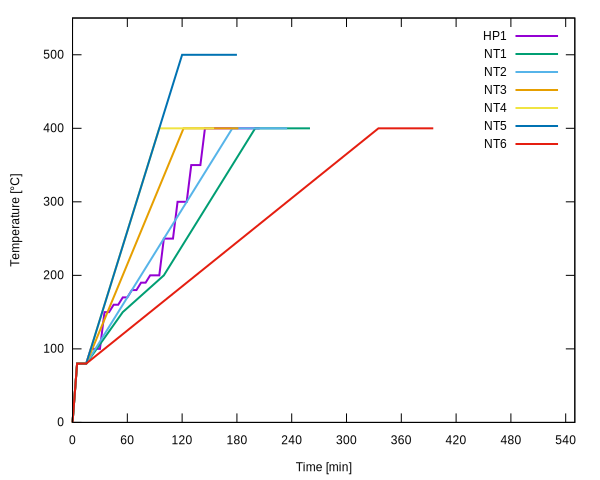
\includegraphics[width=.7\textwidth]{../Data/Graphs/hp1.png}
%	\caption{Different heatings curves}
%	\label{fig:heat}
%\end{figure}

%%%%%%%%%%%%%%%%%%%%%%%%%%%%%%%%%%%%%%%%%%%%%%%%%%%%%%%%%%%%%%%%%%%%%%%%%%%%%%%%%%%%%%%%
%%%%%%%%%%%%%%%%%%%%%%%%%%%%%%%%% CHARACTERISATION %%%%%%%%%%%%%%%%%%%%%%%%%%%%%%%%%%%%%
%%%%%%%%%%%%%%%%%%%%%%%%%%%%%%%%%%%%%%%%%%%%%%%%%%%%%%%%%%%%%%%%%%%%%%%%%%%%%%%%%%%%%%%%
\section{Characterisation}
All \gls{sem} micrographs were taken with a Zeiss Supra 40. 
\Gls{ft}\gls{uv}/\gls{vis}/\gls{nir} transmittance and reflectance spectra (at \SI{20}{\degree} incident 
angle) were recorded with a Bruker Vertex 70 
%transmission [\%] and reflection?  which angle? 
spectrometer with a quartz beam splitter, \SI{0.5}{\milli\meter} aperture and 
Gallium-Phosphide detector for ultra violet light (\SI{303}{\nano\meter}--\SI{588}
% gallium phosphide http://dx.doi.org/10.1051/epjconf/20134800028
{\nano\meter}) and a Silicon detector for visual and \gls{nir} light 
(\SI{500}{\nano\meter}--\SI{1.2}{\micro\meter}). For transmittance the light
entered the sample from the side with the layer. The \gls{uv} and \gls{vis}/\gls{nir} spectra were merged 
in Opus software. % included in the spectrometer. 
\Gls{xrd} spectra were obtained with a Thermo Scientific ARL Equinox 100 X-Ray Diffractometer. 
All \gls{xrd} spectra were taken at \SI{5}{\degree} incident angle and compared to the internal database.

The \gls{iv} curves were measured with Agilent 4156C Precision Semiconductor 
Parameter Analyzer from \SI{-0.5}{\volt} to \SI{0.5}{\volt} with steps of 
\SI{10}{\milli\volt}.
Prior to \gls{iv} measurements the samples were sputtered with aluminium 
through a mask to produce a multitude of equidistant contacts with a Leybold 
UNIVEX450C Sputter System.
Directional current sputtering was used with Argon as inert gas at \SI{0.005}{\milli\bar} 
and with a power of \SI{40}{\watt} for \SI{700}{\second}.
Between sputtering and \gls{iv} measurements 
direct contacts to the steel substrate were created by removing a patch of the \gls{zro}
layer with 
sand paper on two opposing edges of a sample and then by applying silver paste.
See figure~\ref{fig:circuit} for a sketch of the connectivity.

\begin{figure}[hbt]
    \centering
    \begin{circuitikz} \draw
        (0,0) to[european voltage source] (0,2)
        to[ammeter] (2,2) 
        to[generic,l=W] (4,2) 
        to[generic,l=Au] (6,2) 
        to[generic,l=Al] (8,2)
        -- (8,2)
        to[generic,l=ZrO$_2$] (8,0)
        -- (8,0)
        to[generic,l=steel] (6,0)
        to[generic,l=Ag] (4,0)
        to[generic,l=Au] (2,0) 
        to[generic,l=W] (0,0) 
            ;
    \end{circuitikz}
    \caption{Sketch of circuit, from the source clockwise: varibale voltage source, built-in amperometer, gold plated tungsten probe, sputtered aluminium contact, \gls{zro} layer to be measured, steel substrate, dried silver paste contact, gold plated tungsten probe.}
    \label{fig:circuit}
\end{figure}

%%%%%%%%%%%%%%%%%%%%%%%%%%%%%%%%%%%%%%%%%%%%%%%%%%%%%%%%%%%%%%%%%%%%%%%%%%%%%%%%%%%%%%%%
%%%%%%%%%%%%%%%%%%%%%%%%%%%%%%%%%%% PREOPTIMISATION %%%%%%%%%%%%%%%%%%%%%%%%%%%%%%%%%%%%
%%%%%%%%%%%%%%%%%%%%%%%%%%%%%%%%%%%%%%%%%%%%%%%%%%%%%%%%%%%%%%%%%%%%%%%%%%%%%%%%%%%%%%%%
\section{Pre-optimisation}\label{sec:exp-preopt}
%\td{the choice of grenzen for \gls{doe} was done by biotic reinforcement learning (i.e. my brain)}
%\td{Screening}
%The main part of the screening pre-optimisation samples were optimized via biotic reinforcement learning (i.e. my brain). 
The main part of all samples (around 90\%) were pre-optimization samples, 
from which the bulk were screening experiments optimized via biotic reinforcement learning 
(i.e. my brain) in order to obtain reasonable constraints for computerized pre-optimization. 
%Initially, glass plates were doctor bladed manually with aquatic solution and calcinated 
%via HP1. 
%Glass was used because of its availability and in order to be able to make IR 
%\td{transmission} spectra.
%In order to measure the resistivity of the produced layer \gls{fto} and \gls{ito} layered 
%glass plates (both conductive) were used as substrate.
%Conducting substrates were also needed to produce \gls{sem} micrographs. 
%\td{should maybe put this into beginning of section \ref{sec:exp}?}
%otherwise the sample would charge and can't be pictured anymore. 
%this means if the produced layer is thick and homogeneous enough, it's difficult to see in sem
%Different additives were included in the recipe (see table \ref{tab:rec1}) and the resistance was checked with a multimeter. 
%\todo{different additives, heating programs (NT1-NT5 and HP1), blade distances (distance between blade and substrate) and layer counts were tried}
Composition of the aquatic solution, heating program, blade distance (distance between 
blade and substrate) and layer count were varied but no homogeneous layers resulted. 
Thus, 
the buthanolic recipe was introduced, which gave rise to homogeneous films.
After the blade moved over the substrate the remaining liquid needed about a minute 
to evaporate. 
%\td{
The then current procedure resulted in clear and continuous films, but was plagued from 
inhomogeneities due to drying stains. 
The drying stains could be circumvented by using a heat gun, but the results were not 
reproducible. 
The glass plate of the film applicator was therefore exchanged with a metal plate which 
allowed to hold the sample in place through underpressure and simultaneously heat it to a certain 
temperature. The bounds of the process variables were then explored in a preliminary study 
using the Plackett-Burman\cite{Plackett1946} design implemented in the \texttt{python3} 
library \texttt{pyDOE}. With 
(1,5), (4,10), (400,500), (120,480), (0.1,5) and  (20,80) 
as nominal and extreme values for 
relative concentration of Zr $c_{zr}$, number of layers $\lambda$, calcination temperature $T_{cal}$[\oc{}], heating rate $v_{cal}$[\oc{}/\h{}], \gls{db} velocity $v_{DB}$[\mm{}/\s{}] and \gls{db} temperature $T_{DB}$[\oc{}], respectively. 
After testing the first samples, the lower limit for \gls{db} velocities was altered from 0.1 to 1 (see table \ref{tab:pre-opt1}).
\begin{table}[hbt]
	\centering
	\caption{Pre-optimization experiments}
	\label{tab:pre-opt}
	\begin{subtable}{0.5\linewidth}
		\centering
		\subcaption{Placket-Burman style experiments}
		\label{tab:pre-opt1}
		\begin{tabular}{cccccc}
			\hline
			\hline
	%		&80-150\oc{} [\oc{}/\minutes{}]	&150-200\oc{} [\oc{}/\minutes{}]	&200\oc{}-T$_{\textrm{Cal}}$ [\oc{}/\minutes{}]	&T$_{\textrm{Cal}}$ [\oc{}] &t$_{\textrm{Cal}}$ [\minutes{}]	\\
			$c_{zr}$	&$\lambda$	&$v_{DB}$	&$T_{DB}$	&$v_{cal}$	&$T_{cal}$		\\
			\hline
	1	&10	&5	&20	&120	&400	\\
	1	&4	&0.1	&20	&120	&500	\\
	5	&10	&0.1	&20	&120	&500	\\
	5	&4	&5	&20	&480	&400	\\
	1	&5	&5	&80	&120	&500	\\
	1	&10	&1	&80	&480	&400	\\
	5	&5	&1	&80	&120	&400	\\
	5	&10	&5	&80	&480	&500	\\
			\hline\hline
		\end{tabular}
	\end{subtable}%
	\begin{subtable}{0.5\linewidth}
		\centering
        \subcaption{Hand picked experiments; $^*$varied stabilisation agent}
		\label{tab:pre-opt2}
		\begin{tabular}{cccccc}
	%conc	&layers	&vDOC	&TDOC	&vCal	&Tcal		\\
			\hline\hline
			$c_{zr}$	&$\lambda$	&$v_{DB}$	&$T_{DB}$	&$v_{cal}$	&$T_{cal}$		\\
	%conc	&layers	&$v_{\textrm{DB}}$	&$T_{\textrm{DB}}$	&$v_{\textrm{cal}}$	&$T_{\textrm{cal}}$		\\
			\hline
	2	&8	&0.5	&40	&360	&470	\\
	2	&6	&2	&40	&360	&430	\\
	1	&4	&12	&70	&120	&500	\\
	1	&9	&18	&80	&240	&400	\\
	4$^*$	&6	&14	&60	&240	&500	\\
%	4$^\dagger$	&6	&14	&60	&240	&500	\\
%	4$^\ddagger$	&6	&14	&60	&240	&500	\\
			\hline
			\hline
			\\ \\  \\
%			\multicolumn{6}{c}{*different stabilisation reagent compositions}\\
		\end{tabular}
	\end{subtable}
\end{table}

%$T_{DB}$[\oc{}]
%$v_{DB}$[\mm{}/\s{}]
%$T_{cal}$[\oc{}]
%$v_{cal}$[\oc{}/\h{}]
%Especially the doctor blading velocity.
%}
%It was tried to reduce the waiting time and the resulting \td{drying stains}
%by using a heat gun. The drying was
%accelerated but not reproducibly and the glass plate on the film applicator was changed 
%against the heatable plate.
%With this new buthanolic recipe and heatable plate the limits of the optimization problem 
%were explored in a preliminary study using the Plackett-Burman \cite{Plackett1946} design 
%implemented in the \texttt{python3} library \texttt{pyDOE}.
%For the preliminary study a DB machine and NT were used and the steel. 
\ds{In the preliminary study only steel was used as substrate.}
%The Plackett-Burman \cite{Plackett1946} design implemented in the python3 library \texttt{pyDOE} was used to
%get an overview of reasonable boundaries.
%Latin squares were used to chose which experiments should be ausgefuehrt to get an ueberblick of the optimization room.
%See Code/Input_DOE/make_*exps.py and Code/Input_DOE/mail_theo
Some additional hand picked experiments (see table \ref{tab:pre-opt2}) were introduced to further narrow down the limits of 
the optimization as every reduction in variables or levels meant a faster convergence.
%ooooh 
%%%%%%%%%%%%%%%%%%%%%%%%%%%%%%%%%%%%%%%%%%%%%%%%%%%%%%%%%%%%%%
Shortly before the \gls{pso} the stabilisation agent was changed from \gls{acoh} to 
\gls{ipo} because of much better solution stability.
The - up to this moment - best process was chosen to be tested with 
\ml{1} \gls{acoh}, \ml{0.5} \gls{acoh} plus \ml{0.5} \gls{ipo} and \ml{1} \gls{ipo}.
%\td{As the sample showed the best all ex were proceeded with ipo as stabilisation agent. }
The sample produced with \gls{ipo} as stabilization agent 
showed comparable passivization results and better stability. 
Therefore \gls{ipo} was used  as stabilisation in further experiments.
After the boundaries of the solution were fixed 
the process variables to produce an insulating layer was examined. 
%There were many variables which had to be taken into account. 
%\td{plachett-burman design of experiment with conc, layers, calcination temperature, heating rate, DB velocity and DB temperature as input variables.}
See table \ref{tab:space} for the space spanned for the optimisation.
\begin{table}[ht!]
	\centering
	\caption{Final values used in the \gls{pso}.}
    \label{tab:space}
    \begin{tabular}{cccccc}
        \hline\hline
		$c_{zr}$	&$\lambda$	&$v_{DB}$	&$T_{DB}$	&$v_{cal}$	&$T_{cal}$		\\
%        concentration   &layers &\gls{db} velocity  &\gls{db} temperature   &heating rate   &calcination temperature    \\
        \hline
        2   &4  &10 &40 &120    &300    \\
        3   &6  &12 &50 &360    &400    \\
        4   &8  &14 &60 &600    &500    \\
        5   &10 &16 &70 &840    &       \\
            &12 &18 &80 &1080   &       \\
            &   &20 &   &       &       \\
        \hline\hline
    \end{tabular}
\end{table}

\ds{The final boundaries were
conc 2 - 5 (1) ,
layers 4 - 12 (2),
\gls{db} velocity 10 - 20 (2),
\gls{db} temperature 20 - 80 (20),
heating rate 120 - 1080 (240),
calcination temp 300 - 500 (100),
.
}


\clearpage

%%%%%%%%%%%%%%%%%%%%%%%%%%%%%%%%%%%%%%%%%%%%%%%%%%%%%%%
%%%%%%%%%%%% 5 COMPUTATIONAL DETAILS %%%%%%%%%%%%%%%%%%
%%%%%%%%%%%%%%%%%%%%%%%%%%%%%%%%%%%%%%%%%%%%%%%%%%%%%%%
\section{Computational Details}
\label{sec:comp}
%\subsection{Data Processing}
\label{sec:eval}
Reading list
\begin{itemize}
    %\item https://de.wikipedia.org/wiki/Globaler_F-Test
    %\item https://de.wikipedia.org/wiki/Optimale_Versuchsplanung
    %\item Curse of dimensionality scholar
    %\item linear regression von ungar 
    %\item ridge regression + support vector machine
    %\item correlation vs covariance
    %\item https://en.wikipedia.org/wiki/Regression_analysis
    %\item https://en.wikipedia.org/wiki/Noise_reduction
    %\item https://en.wikipedia.org/wiki/Feature_extraction
    %\item https://en.wikipedia.org/wiki/Feature_selection
    %\item https://en.wikipedia.org/wiki/Dimensionality_reduction
    %\item file:///home/pur/Doc/Uni/Chemie_Master/Int_AIT/Int.git/Code/ML/98_things_can_go_wrong_in_ML_project.html
    %\item https://scikit-learn.org/stable/modules/generated/sklearn.decomposition.PCA.html
    %\item https://scikit-learn.org/stable/modules/generated/sklearn.decomposition.KernelPCA.html#sklearn.decomposition.KernelPCA
    \item 
    \item 
    \item 
\end{itemize}
%\td{describe problem and solution found}
For every sample multiple \gls{iv} curves were measured. 
The main difficulty faced in processing the data was to present the measurements obtain 
from a sample in one representative number. 
The average of each conductance would be an obvious choice but difficult to represent a 
sample correctly since the possible values of conductance span accross several magnitudes.
So the average of logarithms of conductances is the next nearby ansatz.
\todo{why didn't i just take this?}
\td{L2 norm because it might be easier to compare to other methods. }
\td{inspired by euclidean norm/L2 distance from ideal case} 
\td{wanted to put more weight on bad shunts}
\td{plot avg, avg(log), avg(log-13)}

For every I-V curve (aluminium dot) the gradient $g$ at $V=0$ is calculated by taking 
each $n=5$ points after and before the origin at least $d=2$ points distance (which boils
down to the values from \SI{0.02}{\volt} to \SI{0.07}{\volt}) , averaging their V and I values 
and calculating
\begin{equation}
    g = \frac{I_{+m+d} - I_n}{V_{n+1} - V_n}.
\end{equation}
As a measure of conductance a distance D from an ideal non-conducting case. The average of the negative base 10 logarithm subtracted from an ideal non-conducting gradient of $10^{-13}$ 
\begin{equation}
	D = \sum_i^N \frac{ -log_{10}(g_i) - 13}{N}
	\label{eq:D}
\end{equation}
Another measure is the density of shorted species $\rho_{s}$ is calculated in following way:
\begin{equation}
	s_i = \begin{cases}
	1 &\text{if} \quad -log(g_i) < 5 \\
	0 &\text{if} \quad -log(g_i) \geq 5 \\
	\end{cases}
\end{equation}
\begin{equation}
	\rho_s = \sum_i^N \frac{s_i}{N}
	\label{eq:rho}
\end{equation}
Other estimates of the conductance are the averages:
\begin{equation}
	G_1 = log \left( \sum_i^N \frac{g_i}{N} \right)
\end{equation}

\begin{equation}
	G_2 =  \sum_i^N \frac{log(g_i)}{N}
\end{equation}

\subsection{Sample Selection}
\label{sec:ss}
An evolutionary approach was chosen, namely a multi-objective Particle Swarm Optimization (PSO) with a multi-response
Multivariate Adaptive Regression Splines (MARS) model\cite{Villanova2010,Kennedy1995,Breiman1997,Carta2011}.
%
"PSO is a population based heuristic inspired by the flocking behavior of birds. 
To simulate the behavior of a swarm, each bird (or particle) is allowed to fly towards the optimum solution."\cite{Villanova2010}
%
Initially the input parameters (independent variables), their boundaries and number of equidistant levels for each parameter are declared (see table \ref{tab:input}).
Next, the output variables (dependant variables), their weights in the objective function (the function which should be optimized) are specified and if they should be minimized or maximized is noted.
%
%An initial population of particles, i.e. experiments with certain parameters, is chosen out of the population space (space spanned by all possible combinations of input parameters), 
\begin{table}[htb]
	\centering
	\begin{tabular}{cc cc cc}
		\hline
		Zr(PrO)$_4$ conc. [21 g/L]	&layers	&$T_{DB}$[\oc{}]	&$v_{DB}$[\mm{}/\s{}]	&$T_{cal}$[\oc{}]	&$v_{cal}$[\oc{}/\h{}]	\\
		\hline
		2				&4		&40					&10				&300				&120	\\
		3				&6		&50					&12				&400				&360	\\
		4				&8		&60					&14				&500				&600	\\
		5				&10		&70					&16				&					&840	\\
						&12		&80					&18				&					&1080	\\
						&		&					&20				&					&		\\
		\hline
	\end{tabular}
	\caption{Discrete levels of each input parameter \td{are concentrations correct?}}
	\label{tab:input}
\end{table}

The first step is to select an initial population (ensemble of experiments), which is chosen randomly from the population space. 
The samples are made, measured and evaluated according to section \ref{sec:exp} and the distance $D$ (see eq. \ref{eq:D}), $\rho_s$ (see eq. \ref{eq:rho}), $n_{layers}$ (numbers of layers) and $v_{cal}$ (heating rate of calcination process in \oc{}/\minutes{}) are supplied to the program. 
The program uses this data to estimate a response for each output variable (and to choose a fraction of the initial population which is allowed to propagate).
The response variables for the entire population space is calculated. 
The current population - each of the particles independently - moves towards the optimum solution.
The population for the next time step is outputted and the experiments are again executed, measured and evaluated.

\td{system behavior are discussed in Modeling the Results.
Algorithm and Coating Features. The theoretical efficiency
of the proposed approach has been verified using a simulation
based on a preliminary experimental model (48 recipes evalu-
ated, see the Supporting Information, S3). Then, 15 new experi-
ments were selected for each subsequent time instant. Each time
instant involves experiment identification, solution preparation,
coating deposition, and spot analysis.
Figure 2a presents the laser scanner measurement of a spot
}\cite{Carta2011}
%\subsection{EMMA Propagation}
%\begin{table}[htb]
%	\centering
%	\begin{tabular}{ccccccc}
%		\hline
%		\hline
%conc	&layers	&vDOC	&TDOC	&vCal	&Tcal	&	\\
%		\hline
%1	&10	&5	&20	&120	&400	&\\
%1	&4	&0.1	&20	&120	&500	&\\
%5	&10	&0.1	&20	&120	&500	&\\
%5	&4	&5	&20	&480	&400	&\\
%1	&5	&5	&80	&120	&500	&\\
%1	&10	&1	&80	&480	&400	&\\
%5	&5	&1	&80	&120	&400	&\\
%5	&10	&5	&80	&480	&500	&\\
%2	&8	&0.5	&40	&360	&470	&\\
%2	&6	&2	&40	&360	&430	&\\
%		\hline
%%4	&12	&-	&-	&-	&-&\\
%1	&4	&12	&70	&120	&500	&\\
%1	&9	&18	&80	&240	&400	&\\
%%2	&5	&18	&70	&-	&-		&\\
%4	&6	&14	&60	&240	&500	&\\
%4	&6	&14	&60	&240	&500	&\\
%4	&6	&14	&60	&240	&500	&\\
%		\hline
%2	&10	&20	&40	&120	&500	&6113\\
%3	&8	&18	&70	&1080	&300	&2850\\
%3	&6	&10	&50	&1080	&400	&5526	\\
%%3	&10	&14	&50	&600	&500	&-7374	\\
%3	&10	&16	&80	&120	&500	&6554	\\
%4	&6	&16	&80	&1080	&300	&2947	\\
%3	&12	&12	&80	&840	&500	&8318	\\
%3	&10	&14	&50	&600	&500	&7374	\\
%5	&6	&10	&60	&1080	&400	&5648	\\
%5	&10	&20	&60	&360	&300	&3956	\\
%5	&12	&14	&60	&1080	&300	&2700	\\
%		\hline
%%2	&2	&10	&40	&600	&300	&-7201	\\
%2	&4	&10	&80	&1080	&300	&6101	\\
%%2	&4	&10	&40	&600	&300	&-7201	\\
%2	&4	&10	&40	&600	&300	&7201	\\
%3	&4	&12	&60	&600	&300	&1462	\\
%4	&4	&10	&80	&1080	&300	&2883	\\
%5	&12	&20	&70	&600	&300	&1680	\\
%		\hline
%2	&4	&10	&40	&120	&300	&1	\\
%2	&4	&10	&40	&120	&500	&6001	\\
%3	&4	&10	&40	&120	&500	&6102	\\
%5	&4	&10	&80	&1080	&300	&2884	\\
%5	&12	&20	&60	&120	&300	&360	\\
%		\hline
%3	&4	&10	&40	&600	&400	&4202	\\
%2	&6	&20	&40	&120	&500	&6105	\\
%%4	&4	&14	&80	&1080	&300	&-2923	\\
%5	&12	&14	&60	&600	&300	&1500	\\
%3	&6	&14	&60	&600	&300	&1486	\\
%4	&4	&14	&80	&1080	&300	&2923	\\
%		\hline
%4	&8	&18	&80	&1080	&300	&2971	\\
%3	&8	&10	&50	&1080	&300	&2530	\\
%2	&12	&16	&40	&120	&400	&3077	\\
%2	&10	&18	&60	&1080	&300	&2733	\\
%4	&10	&10	&50	&1080	&300	&2535	\\
%		\hline
%		\hline
%	\end{tabular}
%	\caption{}
%	\label{tab:emma}
%\end{table}
%


\subsection{Fitting via Machine Learning}
\td{scarce data may lead to overfitting\cite{Lecun1995conv}}\\
Python and sci-kit learn \td{cite} was used to implement a linear fit model, and SVR with the kernels polynomial, rbf and sigmoid. 
The space of hyper parameters C, the degree (in case of polynomial), epsilon and gamma was scaned. 

The independent variables are located on a partially irregular grid.  


%\clearpage

%%%%%%%%%%%%%%%%%%%%%%%%%%%%%%%%%%%%%%%%%%%%%%%%%%%%%%%
%%%%%%%%%%%%%% 6 RESULTS AND DISCUSSION %%%%%%%%%%%%%%%
%%%%%%%%%%%%%%%%%%%%%%%%%%%%%%%%%%%%%%%%%%%%%%%%%%%%%%%
\section{Results and Discussion}
\label{sec:results}
%%%%%%%%%%%%%%%%%%%%%%%%%%%%%%%%%%%%%%%%%%%%%%%%%%%%%%%%%%%%
and cite something pro forma \cite{ncbi1butanol}
%
%%%%%%%%%%%%%%%%%%%%%%%%%%%%%%%%%%%%%%%%%%%%%%%%%%%%%%%%%%%
%%%%%%%%%%%%%%%%%%%%%%%%%%%%%%%%%%%%%%%%%%%%%%%%%%%%%%%%%%%
\subsection{XRD}
\begin{figure}
	\centering
	\includegraphics[width=\picwidth]{Pics/xrd.png}
	\caption{XRD spectra}
	\label{fig:xrd}
\end{figure}

%%%%%%%%%%%%%%%%%%%%%%%%%%%%%%%%%%%%%%%%%%%%%%%%%%%%%%%%%%%
%%%%%%%%%%%%%%%%%%%%%%%%%%%%%%%%%%%%%%%%%%%%%%%%%%%%%%%%%%%
\subsection{SEM}

%%%%%%%%%%%%%%%%%%%%%%%%%%%%%%%%%%%%%%%%%%%%%%%%%%%%%%%%%%%
%%%%%%%%%%%%%%%%%%%%%%%%%%%%%%%%%%%%%%%%%%%%%%%%%%%%%%%%%%%
\subsection{Material Scientific}
\subsubsection{First recipe} 
alteration of pH etc no improvement 

\subsubsection{Stability of the Solution}
\begin{itemize}
    \item compare AcOH vs AcOH+IPO 1:1 vs IPO (via boxplot) also G and phd? 
    \item p68 solution became clear after being milky 
    \item p74 
    \item why does IPO stabilize? 
    \item what is the reason for instability? 
    \item why does increased Zr conc decrease stability
    \item initial stirring time no influence on stability (and resulting layer?)
\end{itemize}

%%%%%%%%%%%%%%%%%%%%%%%%%%%%%%%%%%%%%%%%%%%%%%%%%%%%%%%%%%%
\subsubsection{Material}
\td{show results between 1ml acoh (199), acoh+ipo 1:1 (201) and ipo (192). Show graph of the three vs log pondus G and pinhole density and maybe distribution of single point measurements?}
\td{p68 iPrOH to milky solution and solution becomes clear!!!! checked how much 
is needed. 5F solution milky over night ~2ml, added 1ml IPO and clear.}
\td{instead of changing the stabilisation agent before optimisation, could change after pso, was vor und nachteile?}
\td{
so higher concentration of zro2 leads to less stable solution
5F ca 100min
4F ca 140min
3F ca 420min (7h)
}
- aquatic vs buthanolic: aquatic immidiately milky
\texttt{set boxwidth 2; set xtics 5; p "stat.dat" u 1:3 with boxes} 
\begin{itemize}
    \item double calcination (2x400C) was tried instead of pyrolization (4x200 then 400C),p49
\end{itemize}

%%%%%%%%%%%%%%%%%%%%%%%%%%%%%%%%%%%%%%%%%%%%%%%%%%%%%%%%%%%
%%%%%%%%%%%%%%%%%%%%%%%%%%%%%%%%%%%%%%%%%%%%%%%%%%%%%%%%%%%
\subsection{V-I and preoptimization}
\td{plot the predicted data for variables which should be excluded (Tcal, Vcal,Conc, layers)}
\td{varied doctor blading velocity: 10, 5, 1, 0.5, 0.2, 0.1. Slower less layer}
\todo{Following stirring times (in minutes) were tested and didn't have an influence on stability of the solution: 10-10-20, 10-10-45, 30-30-180.}
\td{extra PB-design with conc(2-4), layers(6-8), tcal(430-470), tvel(4-6),
vdoc(0.5-2), tdoc(40-60). low vdoc very homogenuous but actually nearly no 
deposition because miniscus is pulling liquid off the substrate.}
\td{IPO influence on "stability" p74: 600ul IPO makes clear, 4000 ul BuOH not clear with 
same base solution (1ml of 4F), added extra 400ul to BuOH sol and after 5min clear. 
of 1:5 is unacceptable Dilution }
- 21.8 (1F) from 15.02. 13:30 bis 
26.3 (1ml iPO to ca2ml of 5f) from 16.02. 16:30 bis 18.02.++
18.02 4F in 80min milky
      2F in ca 24h (stabilization AcOH)
- first recipe tried to improve to achieve more restisting layer. by pH value, surface 
tensionand solution ratios (only 10\% change because it was assumed, that the recipe is 
good and should be improved, but the recipe should be altered thoroughly.
two layers were also tried but didn't even pass the visual examination/test/inspection. 
A curst was produced. 
- At this point in time everything was doctor bladed by hand. The hight was varied (with tape).
When the switch to the erichsen was made. The height was kept constant in order to keep 
the variables to optimize ueberschuabar, but could have been even less variables.
If the movement was to slow the resluting  layer would be very inhomogenuous, thus the
velocity wasn't varied.
\td{p75 tested various vDOC (10,15,20) with TDOC (40,60,70,80) variations with only visual 
inspection of evaporation process. Ideally solution evaporate shortly after DB but not 
before} 
n-BuOH has boiling point of ca 117C\td{\cite{ncbi1butanol} look at source}
- p76, 146 (10x1F) good, 154 (3x4F) okay, 156 (3x3F) bad visualisation
- first experiments generated, but trashed because 1F solution neglected, contraints tightened
- p82 test to what extend AcOH can be replaced with iPOH
- 192 was first with IPOH
- why is IPO satbilizing? what are reasons for instability? 
\td{
acceptable layer was produced by buthanolic solution, but very unstable (short lived) how long? p41 
extra AcOH stabilzed but needed so much that dilution too large...
The stirring time was untersucht, but not much difference so shortest was used because 
short time can produces faster and the resulting solution is longer stable 
(after finishing mixing)
10 layers were tried of short stiring and gave good results? samples 130,131,134,135 (p43)
}
- \td{talk about the switch of recipe before emma: makes experiments hard/impossible to compare, but more practical and proof that it works weell} 



%%%%%%%%%%%%%%%%%%%%%%%%%%%%%%%%%%%%%%%%%%%%%%%%%%%%%%%%%%%
%%%%%%%%%%%%%%%%%%%%%%%%%%%%%%%%%%%%%%%%%%%%%%%%%%%%%%%%%%%
\subsection{EMMA}

%%%%%%%%%%%%%%%%%%%%%%%%%%%%%%%%%%%%%%%%%%%%%%%%%%%%%%%%%%%%%%%%%%%%%%%%%%%%%%%%%%%%%%%%5
%\subsubsection{all samples}
A total of 30 recipes (see appendix \ref{sec:app-emma}) have been investigated in 
five iterations ($t = 0, \dots, 4$) of the algorithm. 
Where the first generation encompassed 10 particles and each subsequent generation encompassed 5 particles. 
The best recipes for each generation can be seen in table \ref{tab:emma-Gb}. 
The experiments for generation 5 where not executed but 
predictions were alread made
with the information from the previous generations. 
%%% BEST
The best sample predicted by the algorithm is experiment number 13 with 
lowest solution concentration, second highest layer count, lowest \gls{db} velocity and temperature, 
and lowest calcination heating rate and temperature. 

\begin{table}[htb]
	\centering
    \caption{Global best per generation}
	\label{tab:emma-Gb}
	\begin{tabular}{cccccccc}
        \hline\hline
        generation  &enr &conc &layr &$v_{DB}$ &$T_{DB}$ &$v_{cal}$ &$T_{cal}$\\
        \hline
     1   &1       &2    &4   &10   &40  &120  &300\\
     2   &5       &2    &6   &10   &40  &120  &300\\
     3   &2947    &4    &6   &16   &80 &1080  &300\\
     4   &2405    &2    &6   &10   &40 &1080  &300\\
     5   &13      &2   &10   &10   &40  &120  &300\\
    \hline\hline
	\end{tabular}
\end{table}

\begin{table}
	\centering
    \caption{Predicted G} 
    \label{tab:emma-pred-G}
    \begin{tabular}{cccccc}
        \hline\hline
    enr     &1st gen     &2nd gen        &3rd gen        &4th gen        &5th gen\\
        \hline
    1       &1.214185    &       &       &       &38.7962       \\
    5       &       &4.196626       &       &       &25.47335       \\
    2947    &       &       &10.9594    &       &10.9594       \\
    2405    &       &       &       &20.04962   &25.47335       \\
    13      &       &       &       &       &24.87178   \\
        \hline\hline
    \end{tabular}
\end{table}

%%% OVER TIME 
The only clear trend from table \ref{tab:emma-Gb} is the layer count, which rises with the generations. 
The remaining input variables remained more or less the same except for the 3rd generation. 
%
In table \ref{tab:emma-pred-G} it can be seen that $G$ as predicted 
by the 5th generation by the prediction function lowered with each iteration, 
except for sample 2947, which wasn't predicted but measured. 
This shows that the easiest part of the algorithm, the selection of the optimum 
from predicted values works as expected. 
% and that the predictions included more lower values over time
%
The predicted $G$ for each generation's best as predicted 
by the very generation would increase with each iteration (see table \ref{tab:emma-pred-G}). 
This indicates an underestimation of the $G$ at the beginning and a correction with time. 
%The reason for is probably a 
The underestimation probably stems from a lucky selection of initial experiments. 

In figure \ref{fig:emma-gen} we can see the two measured main target dependent variables, $\gamma$ and $\rho$, of each particle at generations 1 to 4. 
%for each particle included in the optimization. 
%It shows a clear trend which indicates that the optimization worked even though 
Both variables were to be minimized and show a clear trend towards low values indicating 
that the optimization worked even though 
the prediction functions (see equations \ref{eq:emma-G3} - \ref{eq:emma-vcal4}) 
and the chosen samples where not exactly as expected. 
Neither were the measurements for these samples, which might be due to the high measuring error of samples and variation of quality due to uncontrolled independent variables like room temperature or humidity. 

\begin{figure}[hb]
    \centering
    \begin{subfigure}{.45\textwidth}
        \centering
        \includegraphics[width=.8\textwidth]{Pics/stats/gen-G.png}
        \caption{} \label{fig:emma-G-gen}
    \end{subfigure}
    \begin{subfigure}{.45\textwidth}
        \centering
        \includegraphics[width=.8\textwidth]{Pics/stats/gen-phd.png}
        \caption{} \label{fig:emma-phd-gen}
    \end{subfigure}
    \caption{Each $\gamma$ (a) and $\rho$ (b) of each particle and each generation after initial selection process} 
    \label{fig:emma-gen}
\end{figure}

%%% EQUATION 
Equations \ref{eq:emma-G3}-\ref{eq:emma-vcal3} and \ref{eq:emma-G4}-\ref{eq:emma-vcal4} represent the prediction functions at $t=3$ and $t=4$ rounded to 2 significant digits, respectively.
$h(x)$ is the hinge function (also called a rectifier function) of the simple form $h(x) = max(0,x)$. 
The expression $h(\lambda-6)$ translates into layer count only has an influence if larger than 6 
and $h(6-\lambda)$ into layer count influential only if under 6.
%
The first thing to notice is that every prediction function of a generation depends on the same variables. 
%This means that the algorithm must decide on the variables which explain the most variance independent of optimization weights.
This stems from the fact that the algorithm must chose a single minimal set of basis functions to predict all dependent variables. 
%
Knowing this, makes the decision of adding $\lambda$ and $v_{cal}$ as dependent variables rather unfortunate. %highly questionable. 
%As the \gls{mars} algorithm is gready,
Different independent variables compete to be in the prediction functions because of the greediness of the \gls{mars} algorithm. 
%\td{This makes including $\lambda$ and $v_{cal}$ as dependent variables unfortunate decisions with hindsight.}
In equations \ref{eq:emma-phd3} and \ref{eq:emma-G3} the coefficient have the same signs and differ by a factor of roughly 100.
This fits the data well, but the positive influence of the layer count/number is counter intuitive 
as one would expect more layers to be more insulating and thus result in lower conductance and a lower probability of pin holes going all the way trough the \gls{zro} layer. %pin hole density. 
The coefficients of the $v_{cal} \cdot T_{cal}$ interaction in equations \ref{eq:emma-phd3} and \ref{eq:emma-G3} 
seem low, but considering the minimum value of the inter action of \num{36000} should not be under estimated. 
%It's positive the hinge
It is astonishing that the knot of the hinge function for equations \ref{eq:emma-phd3}-\ref{eq:emma-vcal3} was chosen so low; 
basically only including the influence of $\lambda=4$.
On the positive site the calcination heating rate $v_{cal}$ (see equation \ref{eq:emma-vcal}) has been predicted perfectly within numerical precision. 

For each generation the \gls{mse} was calculated such that only samples were used which were available at that time. 
It is 64, 158, 54 and 50 for $t=1,2,3,4$, respectively. 
The high \gls{mse} can be explained because the prediction function is only a constant at $t=2$. 
Appart from the second generation the \gls{mse} falls over time, which might be attributed to overfitting.
The \gls{mse} for each generation was calculated between predicted values for pre-optimisation samples to check for overfitting, 
but the the error sank with each generation (except for the second gen): 102, 118, 58, 50, respectively for $t=1,2,3,4$. 

It is interesting that although prediction functions for $t=3$ perfectly predicted $v_{cal}$ 
the combined \gls{mse} for $t=4$ is lower. 
%%% MAIN INFLUENCE 
%Even without considering the large maximum of $T_{cal}$, 

\iffalse
The coefficient for $T_{cal}$ is the largest for all equations. 
Factoring in the large maximum value of $T_{cal}$ in contrast the other independent variables, 
$T_{cal}$ has the by far the largest influence on the dependent variables. 
The coefficient of the interaction of $layr$ and $T_{cal}$ is about a tenth in size, %interaction between?H
but has the extra factor of $layr$ of up to 12, resulting in the products being in the same order of magnitude.
I can be noted that the coefficient of the $layr\cdot T_{cal}$ interaction always has contrary sign to $T_{cal}$ coefficient. 
%%% EXPECTATION
It should be doubted, though, that the $layr$ only appears as interaction term 
together with $T_{cal}$ and $T_{DB}$, which seems rather than an artefact. 
\fi

\begin{align}
%
%    \label{eq:emma-phd1}
%    \hat{\rho}_1 &= -26  + 0.0025 \cdot T_{DB}\cdot T{Cal}  +  0.056 \cdot  h(6-\lambda)\cdot T_{Cal} \\
%    \label{eq:emma-G1}
%    \hat{\gamma}_1 &= -0.52 + 2.3\cdot 10^{-5} \cdot  T_{DB}\cdot T_{Cal} + 0.00080 \cdot h(6-layr)\cdot T_{cal}\\
%    \label{eq:emma-layr1}
%    \hat{\lambda}_1 &= 7.1 + 8.1\cdot 10^{-5} \cdot T_{DB}\cdot T_{cal} -  0.0056 \cdot  h(6-layr)\cdot T_{cal}\\
%    \label{eq:emma-vcal1}
%    \hat{v}_{cal,1} &= 19 - 0.00025 \cdot  T_{DB}\cdot T_{cal} - 0.0055 \cdot  h(6-layr)\cdot T_{cal}\\
%
%    \label{eq:emma-phd2}
%    \hat{\rho}_2 &= 47\\
%    \label{eq:emma-G2}
%    \hat{\gamma}_2 &= 0.23\\
%    \label{eq:emma-layr2}
%    \hat{\lambda}_2 &= 7.3\\
%    \label{eq:emma-vcal2}
%    \hat{v}_{cal,2} &= 10\\
%
    \label{eq:emma-phd3}
    \hat{\rho}_3 &= 0.075  -   0.0014 \cdot  v_{cal}  +    0.18 \cdot  h(6-\lambda)  + 3.9\cdot 10^{-06} \cdot  v_{cal}\cdot T_{cal} \\
    \label{eq:emma-G3}
    \hat{\gamma}_3 &= 43  -   0.097 \cdot  v_{cal}  +     10 \cdot  h(6-\lambda)  + 0.00026 \cdot  v_{cal}\cdot T_{cal} \\
    \label{eq:emma-layr3}
    \hat{\lambda}_3 &= 9.9  - 0.00064 \cdot  v_{cal}  -     2.7 \cdot  h(6-\lambda)  - 1.3\cdot 10^{-06} \cdot  v_{cal}\cdot T_{cal} \\
    \label{eq:emma-vcal3}
    \hat{v}_{cal,3} &= -5.2\cdot 10^{-15}  +   0.016 \cdot  v_{Cal}  + 1.3\cdot 10^{-15} \cdot  h(6-\lambda)  + 3.9\cdot 10^{-21} \cdot  v_{Cal}\cdot T_{cal} \\
%
    \label{eq:emma-phd4}
    \hat{\rho}_4 &=  -0.87 + 0.0047 \cdot  T_{cal} - 0.00036 \cdot  \lambda\cdot T_{cal}  +  0.0024 \cdot  h(\lambda-6)\cdot T_{DB} \\
    \label{eq:emma-G4}
    \hat{\gamma}_4 &=     -19 + 0.28 \cdot  T_{cal}  - 0.022 \cdot  \lambda\cdot T_{cal}  +  0.16 \cdot  h(\lambda-6)\cdot T_{DB} \\
    \label{eq:emma-layr4}
    \hat{\lambda}_4 &=  6.8 - 0.014 \cdot  T_{cal}  + 0.0018 \cdot  \lambda\cdot T_{cal}  + 0.0060 \cdot  h(\lambda-6)\cdot T_{DB} \\
    \label{eq:emma-vcal4}
    \hat{v}_{cal,4} &=  29 - 0.052 \cdot  T_{cal}  + 0.0011 \cdot  \lambda\cdot T_{cal}  -  0.011 \cdot  h(\lambda-6)\cdot T_{DB} 
\end{align}
%\fi
%what was the best result? For each particle there is best and global best. 

%The calcination heating $v_{cal}$ rate has been predicted perfectly. 
%\td{even though $v_{cal}$ doesn't appear in the prediction function, how is this possible?}
%The number of layers $\lambda$ on the other hand was predicted poorly 
%even though the conversion factor was $1$ and the prediction function dependent on $\lambda$. 


%%%%%%%%%%%%%%%%%%%%%%%%%%%%%%%%%%%%%%%%%%%%%%%%%%%%%%%%%%%%%%%%%%%%%%%%%%%%%%%%%%%%%%%%5
%\subsubsection{how did evolve over time?}


%\iffalse
%\fi

\iffalse
\begin{figure}
\centering
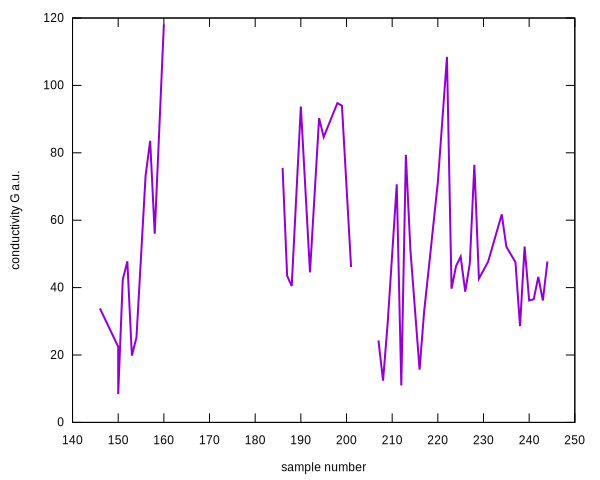
\includegraphics[width=.6\textwidth]{Pics/stats/G-t.png}
    \caption{conductivity G [a.u.] against sample number (is this even correct?)}
    \label{fig:G-t}
\end{figure}

\td{TODO: check if the sorted correctly? Make generation graph with boxplot }
\td{TODO: visualize} how the population moved across the space (with parallel coordinates? or see page 121)
\url{https://stackoverflow.com/questions/30228281/gnuplot-parallel-coordinates-axes-plot-key-annotation}
\fi

%%%%%%%%%%%%%%%%%%%%%%%%%%%%%%%%%%%%%%%%%%%%%%%%%%%%%%%%%%%%%%%%%%%%%%%%%%%%%%%%%%%%%%%%5
%\subsubsection{what is best}
%%%%%%%%%%%%%%%%%%%%%%%%%%%%%%%%%%%%%%%%%%%%%%%%%%%%%%%%%%%%%%%%%%%%%%%%%%%%%%%%%%%%%%%%5
\subsubsection{influence of variable selection on outcome}
The heating rate of the calcination process $v_{cal}$ and the number of layers $\lambda$ were included as dependent variable with the objective to maximize with a relative weight of 0.05 each.
The idea was to maximize $v_{cal}$ and minimize $\lambda$ in order to minimize the process time. 
Another thought behind including $v_{cal}$ and $\lambda$ was to test if the algorithm would correctly predict those. 
%
Three major flaws behind this consideration became obvious with time: 
%
\todo{
(1) The true function for predicting $v_{cal}$ and $\lambda$ are $v_cal*60$ ($C/h$ instead of $C/min$) and $\lambda$, respectively. 
The algorithm will tend to include those values into the prediction function for 
all dependent variables and possibly exclude others which have more influence 
on $\gamma$ and $\rho$ (see equations \ref{eq:emma-G} and \ref{eq:emma-phd}).
%
(2) The algorithm would be influenced by those values to choose samples, which potentially optimize $v_{cal}$ and/or $\lambda$ but not $G$ or $\rho$. 
%
(3) needlessly making the problem more complicate %, important time (around 10\% of the samples) could have been replaced with more insightful samples. 
\begin{itemize}
    \item MARS chooses same set from independent variables for predicting all dependent variables. 
    \item flaws of MARS: all functions are dependent on same independent vars
    \item Every output var is independent of each other, so $v_{cal}$ can act as test 
heating rate was one of the dependent variables with the intention of minimizing the variable. 
It can also be used as test to see how well the EMMA performs (or rather, more precisely MARS)
It doesn't influence the fit for the other splines, but it influences the choice of samples therefore it might have slowed down the process
Overall there were too many variables involved for such a small dataset
        that means that adding dependent variables influences \td{previous variables}
\end{itemize}
}

\td{look at emma papers}
\td{change G to gamma and write enr to every figure}
\td{calculate MSE for predictions}


%\input{chapter/062-discussion.tex}

%\clearpage

%%%%%%%%%%%%%%%%%%%%%%%%%%%%%%%%%%%%%%%%%%%%%%%%%%%%%%%
%%%%%%%%%%%%%%%%%%% 7 OUTLOOK %%%%%%%%%%%%%%%%%%%%%%%%%
%%%%%%%%%%%%%%%%%%%%%%%%%%%%%%%%%%%%%%%%%%%%%%%%%%%%%%%
\section{Outlook}
\label{sec:outlook}
%%\todo{freewriting:} 
%what did i want to do? 
The goal of this work was to find a sol-gel doctor blading process resulting in a insulating zirconium ceramic on top of steel.
This structure then can be used as substrate for thin layer photo voltaics. 
The ceramic needs to be homoegeneous and defect free in order to insulate properly.
%what was done? 
A suitable recipe was found\cite{Hu2016} and the process variables were optimized via \gls{emma}. 
The recipe was improved by increasing its stability. 
The best parameters found by the emma optimization were 
$c_{zr}=2$, $\lambda=10$, $v_{DB}=10$, $T_{DB}=40$, $v_{cal}=120$ and $T_{cal}=300$.
%\todo{$T_{cal}=300$}. 
%welche methoden wurden dafür verwendet? 
After optimzation the data was analysed with further machine learning methods like kernel ridge regression, support vector regression and linear regression. 
The comparisson of methods showed that \gls{emma} performed well on predicting the correlation between conductance and process variables. 
%was wurde herausgefunden? 
A strong correlation of calcination temperature and conductance in the bereich of 300--400\oc{}. 
%was kann noch herausgefundne werden und wie? 
Next steps include to investigate if the correlation of condactance and calcination temperature are statistically significant or due to small sample size. 
The aging process could be examined via infra red spectroscopy. 
%%%%%%%%%%%%%%%%%%%%%%%%%%%%%%%%%%%%%%%%%%%%%%%%%%%%%%%%%%%%%%%%%%%%%%%%%%%%%%%%%%%%%%%5
\iffalse
was kann noch veraendert werden? 
humidity 
solution age
vdb and tdb on g and phd 
Tcal on g and phd 
%%%%%%%%%%%%%%%%%%%%%%%%%%%%%%%%%%%%%%%%%%%%%%%%%%%%%%%%%%%%%%%%%%%%%%%%%%%%%%%%%%%%%%%5

Making of the solution for the sol-gel process:
For a single concentrated solution \ml{0.05} of \gls{zrpro} are added while stirring to \ml{4.95} of \gls{buoh} and stirred for \minutes{15}. 
\ml{0.013} (or one molar equvilent of Zr) of \gls{acac} is added to the stirring solution. 
After another \minutes{15} \ml{1} of acetic acid is added and stirred for \minutes{30} to stabilize the solution up to \h{24}. 

The concentration can be increased up to 5 times being stable for a minimum of \h{4}. 
The sol-gel process produces am homogeneous transparent crystalline zirconia oxide layer. 
homogeneity can be mainly controlled via blade velocity and temperature and layers can be stacked.

It should have been also verglichen with grid search with comparable size
but most time was used to find a vernuenfig base recipe and process

It is still very human 
Der process is - as it the case with all ML and most fitting processes - is very abhaengig von hyper parameters, 
In the current work population size, number of generations, and most importantly boundaries (grenzen). 
\fi

%\clearpage

\bibliographystyle{ieeetr}
\bibliography{int}

\end{document}
